\documentclass[12pt]{article}
\usepackage[slovene]{babel}
\usepackage[utf8]{inputenc}
% \usepackage[T2A]{fontenc}
\usepackage{amsmath}
\usepackage{amsfonts}
\usepackage{amssymb}
\usepackage[version=4]{mhchem}
% \usepackage{stmaryrd}
\usepackage{graphicx}
\usepackage[export]{adjustbox}
\graphicspath{ {./images/} }
\usepackage{physics}
\usepackage{geometry}
\geometry{left=2cm,right=2cm,top=2cm,bottom=2cm}
\usepackage{parskip} 
\usepackage{float}

\title{\textbf{Kotna korelacija anihilacijskih žarkov $\gamma$}}
\author{Samo Krejan}
\date{januar 2026}

\begin{document}
\maketitle

\section{Uvod}

Pozitron $e^+$ se pri srečanju s svojim antidelcem elektronom $e^-$ anihilira. Energija, ki se pri tem sprosti se razširi v prostor v obliki elektromagnetnega valovanja. Zanima nas natančnejša obravnava te anihilacije. Zanima nas ali morda ne pride najprej do nastanka v vodikovem atomu podobne tvorbe v kateri elektron in pozitron krožita okoli skupnega težišča in se anhilirata šele pozneje. Izkaže se, da takšno vezano stanje res obstaja in se imenuje \textbf{positronij}.

V osnovnem stanju positronija sta si delca najbližje skupaj. Kot pri vodikovem atomu ima to stanje orbitalno vrtilno količino l = 0. Glede na to, da imata elektron in pozitron spin 1/2, se osnovno stanje razcepi na singletno stanje z vrtilno količino 0 in tripletno stanje, ki ima vrtilno količino 1. Vezalna energija osnovnega stanja je 6.8 eV. Tripletno stanje je za okoli 1 meV manj vezano od singletnega.

Predpostavimo, da positronij miruje (sicer bi pa obravnavali v $CMS$ in bi nato pretvorili v $LAB$) in da je v singletnem stanju. Ker je vrtilna količina sistema enaka 0, so si v prostoru vse smeri enakovredne. Pri anihilaciji nastali foton lahko torej odleti v katerokoli smer. Zaradi oranjanja vrtilne količine pa mora nastati še en foton, ki odleti v v nasprotno smer. Oba fotona sta ali levo ali desno cirkularno polarizirana.

Za ohranjanje vrtilne količine pri anihilaciji v tripletnem stanju bi potrebovali, da nastanejo najmanj 3 fotoni. To ni tak problem zaradi razlike v življenski dobi obeh sranj. V tripletnem stanju je 1000-krat daljša. V tem času pa pozitronij doživi trke z atomi in iz tripletnega stanja preide v singletno.

Pri vaji se uporablja $^{22}Na$, ki preko $\beta^{+}$ razpada služi kot vir pozitronov. Ta se anihilira z elektronom pri čemer nastaneta dva kolinerarna fotona z energijo $511\ keV$.

\section{Potrebščine}

\begin{itemize}
    \item $^{22}Na$ sevalec,
    \item 2 scintilatorska detektorja,
    \item časovno digitalni pretvornik $Red-Pitaya$,
    \item 2 modula $ORTEC\ 9302$ (ojačevalec in diskriminator),
    \item 8-kanalni razdelilec z zakasnilno enoto $GG800$
\end{itemize}

\section{Naloga}

\begin{enumerate}
    \item Inicializiraj časovno-digitalni pretvornik na plošči Red Pitaya in opravi kalibracijo.
    \item Izmeri ločljivost časovno-digitalnega pretvornika.
    \item Izmeri porazdelitev časovnih intervalov med razpadi radioaktivnega vira.
    \item Poišči koincidence anihilacijskih žarkov $\gamma$ in izmeri njihovo kotno korelacijo.
\end{enumerate}

\begin{figure}[H]
    \begin{center}
        \includegraphics[width=0.8\textwidth]{diagram.png}
    \end{center}
    \caption{Kotna postavitev scintilatorjev.}
    \label{fig:diagram}
\end{figure}

\section{Meritve}

\subsection{Ločljivost TDC-jev}

Za oceno ločljivosti oba TDC-ja priklopimo na isti signal (en izmed scintilatorjev). Ko pomerimo porazdelitev medkanalnih časov, bomo nekje blizu 0 videli oster vrh. V idealnem primeru bi bil tak vrh točno na ničli in bi imel širino 0. V dejanskem primeru dobimo nek spekter. Ločljivost lahko ocenimo kot RMS odmik od idealnega sovpadanja. V programu razberemo, da je ta RMS odmik (oz. standardna deviacija)

\begin{equation*}
    \sigma_t = 2.4\,\mathrm{ns}.
\end{equation*}

\subsection{Enokanalna meritev}

Na obeh TDC-jih pomerimo spekter časov med razpadi. Spektra vidimo na sliki~\ref{fig:random-coincidende}. Če nanju v logaritemski obliki prilagodimo premico, dobimo naklona, ki predstavljata aktivnosti

\begin{align*}
    R_1^{\mathrm{(fit)}} &= (1195 +/- 4)\, \mathrm{s^{-1}}, \\
    R_2^{\mathrm{(fit)}} &= (1408 +/- 5)\, \mathrm{s^{-1}}.
\end{align*}

Na drug način lahko število vseh sunkov pogledamo celokupno in delimo s časom meritve. Pogledamo tudi odstopanja od vrednosti, ki smo jih dobili iz naklona premice.

\begin{align*}
    R_1^{\mathrm{(vse)}} &= 1183\, \mathrm{s^{-1}}, \quad \delta = 0.01, \\
    R_2^{\mathrm{(vse)}} &= 1189\, \mathrm{s^{-1}}, \quad \delta = 0.02.
\end{align*}

Vrednosti, s katerimi bomo nadaljevali račun, vzamemo kar kot sredinsko vrednost obeh metod, za napako pa vzamemo kar odstopanje $\delta$.

\begin{align*}
    R_1 &= (1190 \pm 12)\, \mathrm{s^{-1}}, \\
    R_2 &= (1400 \pm 20)\, \mathrm{s^{-1}}.
\end{align*}

\begin{figure}[H]
    \begin{center}
        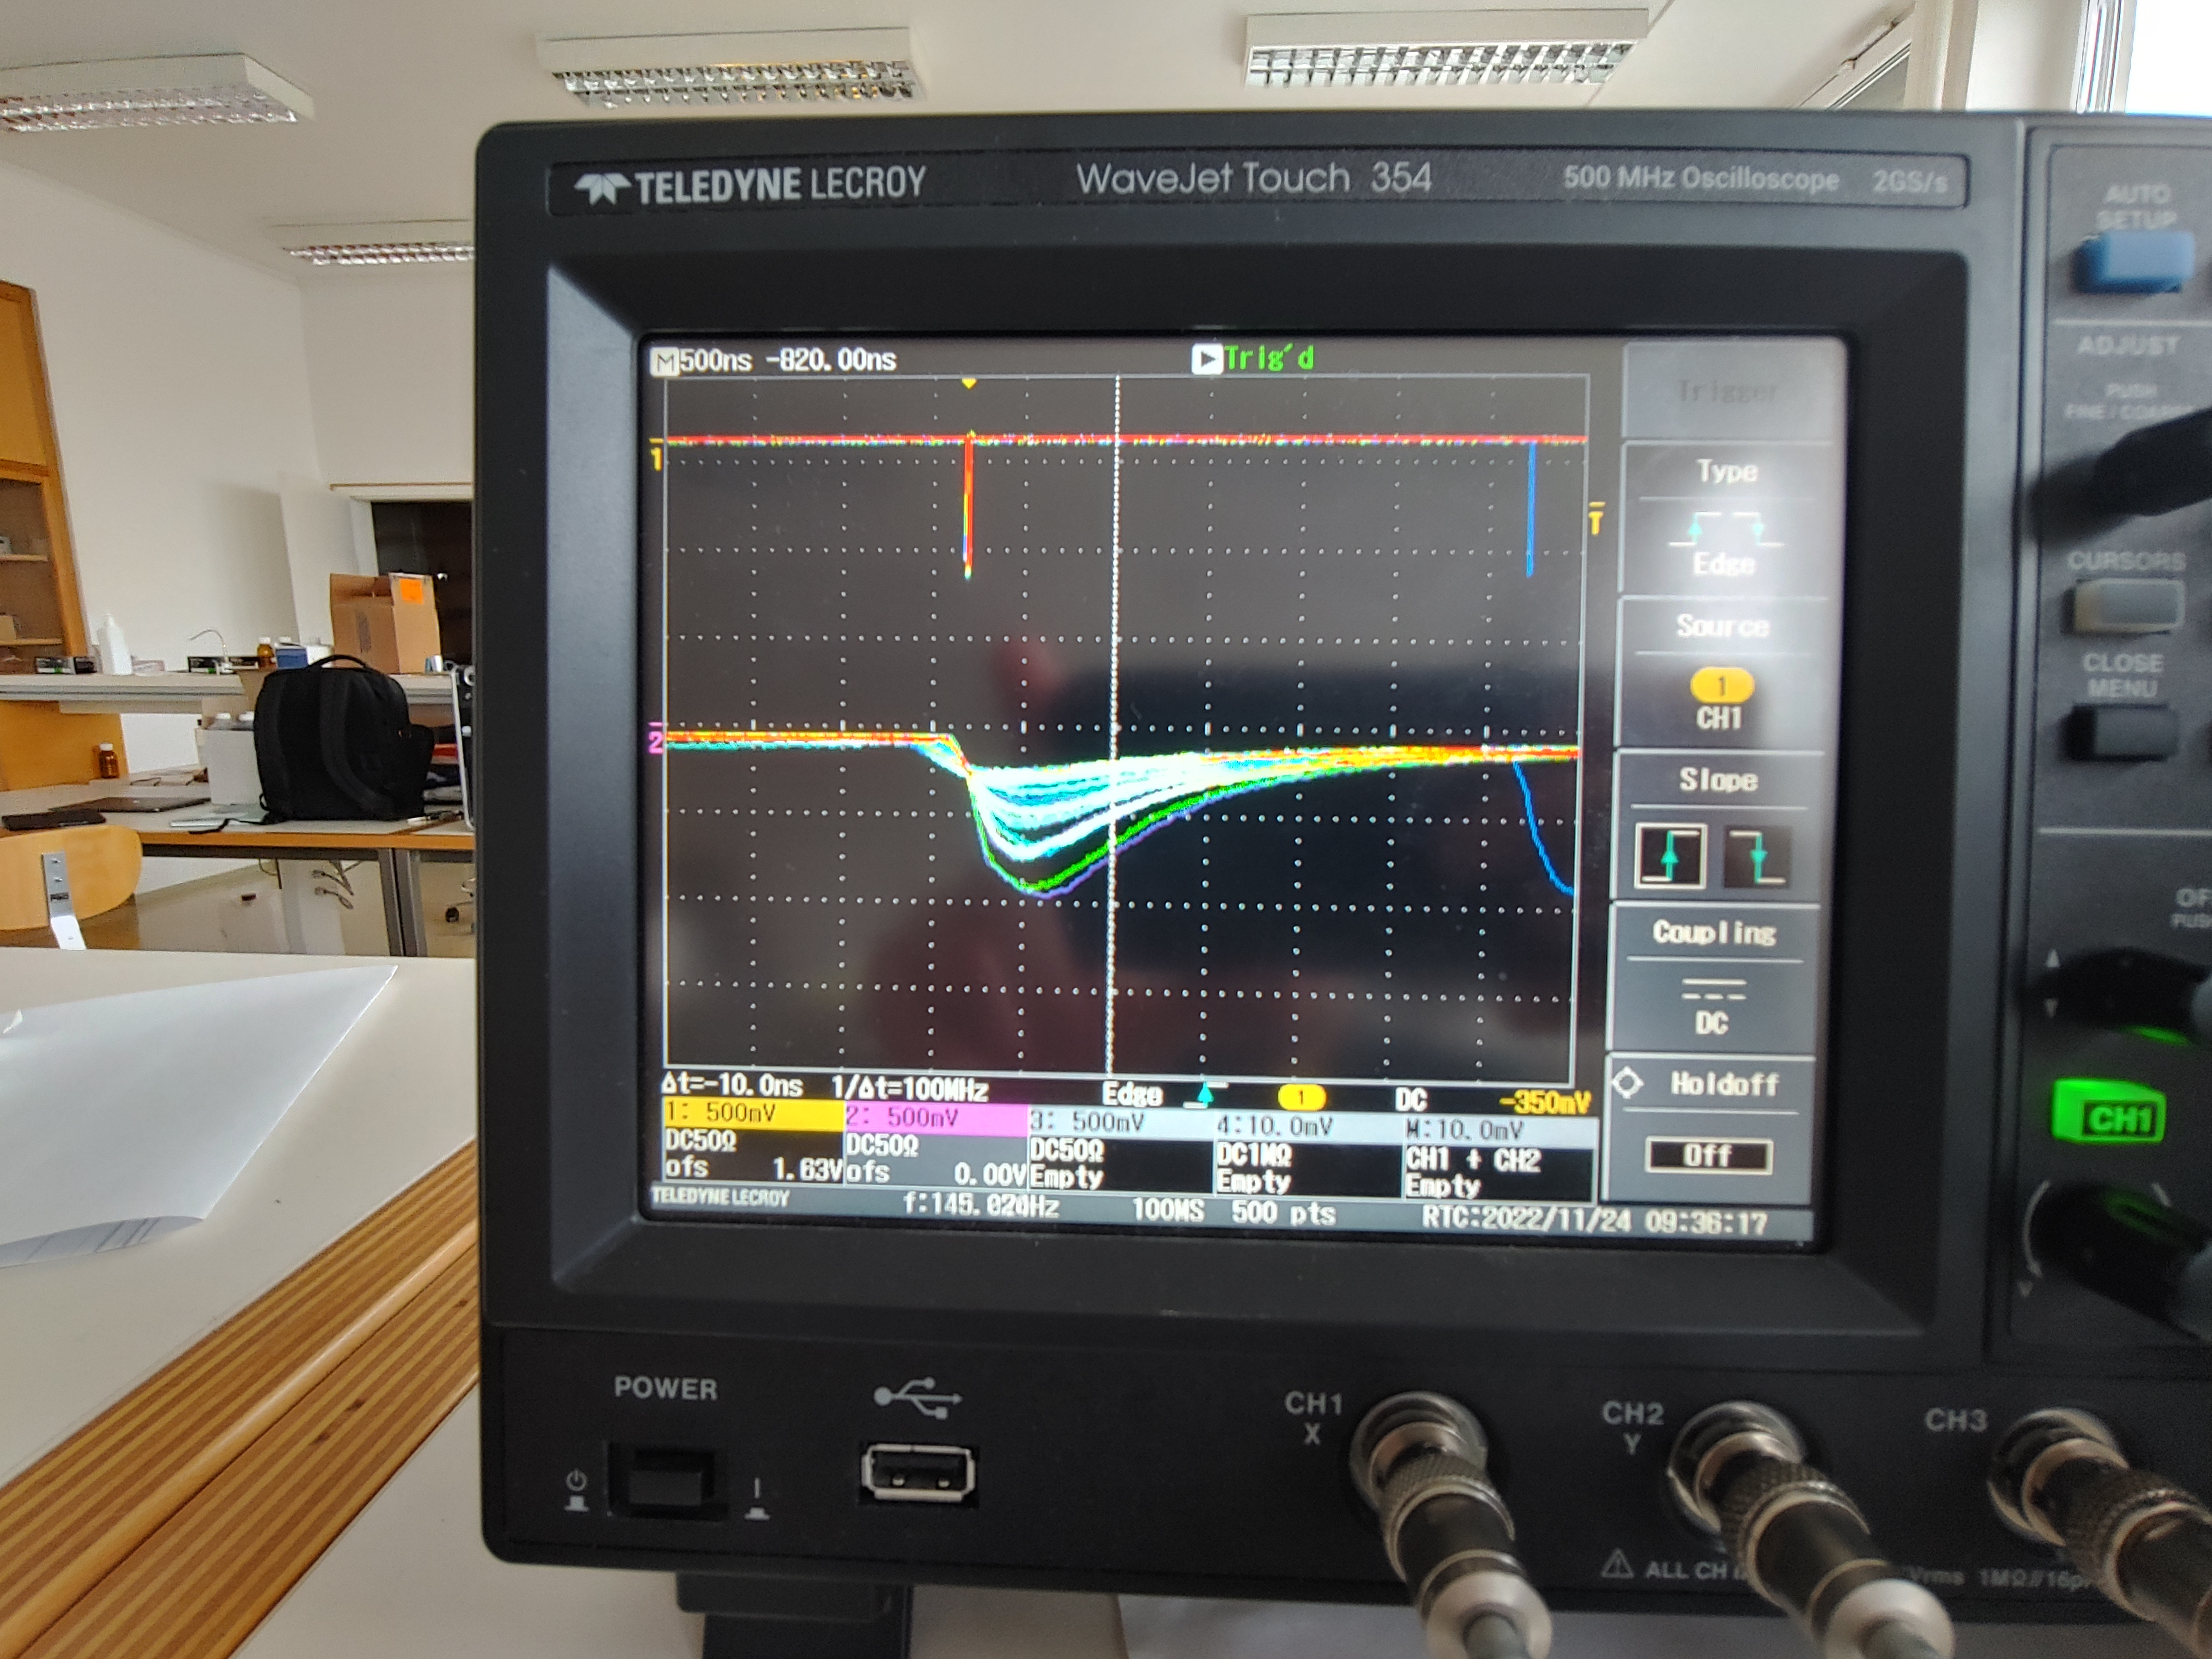
\includegraphics[width=0.49\textwidth]{signal.jpg}
        \includegraphics[width=0.49\textwidth]{width.jpg}
    \end{center}
    \caption{Signali, sunki iz scintilacijskega detektorja na osciloscopu. Amplituda sunka je sorazmerna z energijo elektrona. Na drugi sliki vidimo signale iz diskriminatorja in oblikovalca signalov. Nastavitve so take, da sta oba signala dolga $~100\,\mathrm{ns}$ in da je njih zamik 0.}
\end{figure}

\subsection{Medkanalna meritev}

Zdaj pomerimo porazdelitev medkanalnih časov, prvo pri kotu $180^\circ$~(glej sliko~\ref{fig:diagram}), nato pa še pri nekaj drugih.

Napako števila sunkov ocenimo na nekoliko za lase privlečen način. Na spekter prilagodimo Gaussovko in pogledamo RSS (\textit{ang.} root sum of squares) vrednost odmikov med njo in prilagojenim spektrom.

Razvidno je, da so števila sunkov v celotnem vrhu odvisna od kota med scintilatorjema. Daleč največ sunkov je pri kotu $180^\circ$, tj. pri načinu, ko $\gamma$-fotona odletita v nasprotnih smereh. Tak način razpada označuje singletno stanje.

\begin{figure}[H]
    \begin{center}
        \includegraphics[width=10cm]{correlation.pdf}
    \end{center}
    \caption{Spektri medkanalnih časov v koincidenčnem vrhu za različne kote $\theta$~(slika~\ref{fig:diagram}). S črno so narisane Gaussovke, prilagojene na spekter.}
    \label{fig:correlation}
\end{figure}

\begin{figure}[H]
    \begin{center}
        \includegraphics{correlation-by-angle.pdf}
    \end{center}
    \caption{Odvisnost celokupnega števila sunkov v odvisnosti od kota med scintilatorjema. Kot $180^\circ$ označuje razpad singletnega stanja.}
    \label{fig:by-angle}
\end{figure}

\subsection{Naključne koincidence}

Če obrnemo \verb|DELAY| vijak na eni izmed enot \verb|GG8000|, se koincidenčni vrh odpelje izven merilnega območja, ki smo ga nastavili. Tedaj je zaznana porazdelitev pretežno le še naključne koincidence. Če sta $R_1$, $R_2$ aktivnosti eksponentne porazdelitve, izmerjene na enem in drugem TDC-ju posebej~(slika~\ref{fig:random-coincidende} zgoraj), velja za aktivnost naključni koincidenc produktna zveza

\begin{equation}
    R_{12} = R_1 R_2 \tau,
    \label{eq:product}
\end{equation}

pri čemer je $\tau$ širina merilnega okna $[-500, 500]$. Pričakujemo torej, da bo

\begin{equation*}
    R_{12} = (1.66 \pm 0.03)\,\mathrm{s^{-1}}.
\end{equation*}

A iz medkanalne meritve~(slika~\ref{fig:random-coincidende} spodaj), dobimo aktivnost

\begin{equation*}
    R_{12} = 1.53\,\mathrm{s^{-1}}.
\end{equation*}

Da bi lahko določili napako te druge meritve, bi jo morali nekajkrat ponoviti. Ker pa od naše predvidene vprednosti $(1.66 \pm 0.03)\, \mathrm{s^{-1}}$ odstopa več kot predvideno, sklepam, da je velikostnega reda

\begin{equation*}
    \Delta R_{12} \approx 0.1\,\mathrm{s^{-1}}.
\end{equation*}

\begin{figure}[H]
    \begin{center}
        \includegraphics[width=0.8\linewidth]{random-coincidence.pdf}
    \end{center}
    \caption{Da preverimo zvezo~\ref{eq:product}, izmerimo čase med razpadi na prvem in drugem TDC-ju posebej, nato pa medkanalno izmerimo še naključne koincidence med njima.}
    \label{fig:random-coincidende}
\end{figure}

\end{document}